\chapter{Improvements to the Boosted Analysis}
The boosted analysis described in chapter \cite{chap:anal} is optimized for the case where the ${H\rightarrow b\overline{b}}$ system is boosted and the ${H\rightarrow WW^{*}}$ system is resolved. However, at high resonant masses, one would expect both the ${H\rightarrow b\overline{b}}$ and the ${H\rightarrow WW^{*}}$ to be boosted. However, the semileptonic decay of the W boson pair adds an additional complication of having a lepton within the radius of a large-R jet. This chapter will describe a method for reconstructing this complex topology and the improvements if offers to the boosted, semi-leptonic ${HH\rightarrow b\overline{b}WW^{*}}$ analysis.
\section{Motivation}
The resonant analysis covers a large range of mass hypotheses, from 400 - 3000 GeV. As the resonant mass increases, the two Higgs systems become more and more collimated. Figure ~\ref{fig:dr} shows the average distance between final state partons as a function of the resonant mass for simulated HH events. The $WW$ bosons become very collimated (within dR = 0.5) around 1000 GeV. \newline
\begin{figure}[h]
\begin{center}
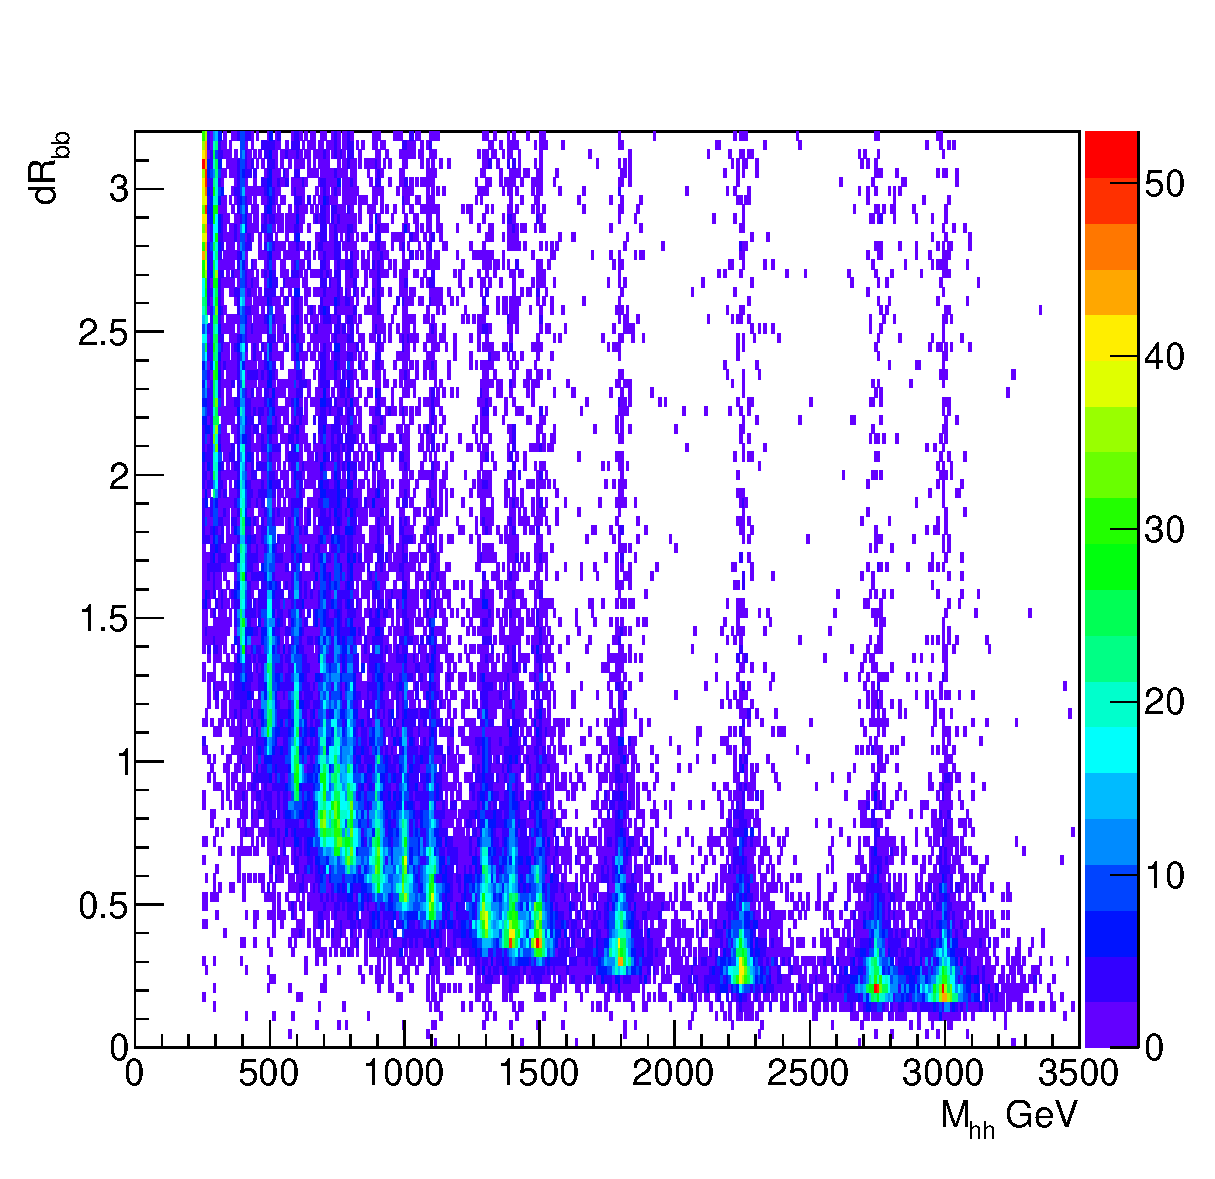
\includegraphics[scale=0.33]{DRMhhPlots_fine/drbb}
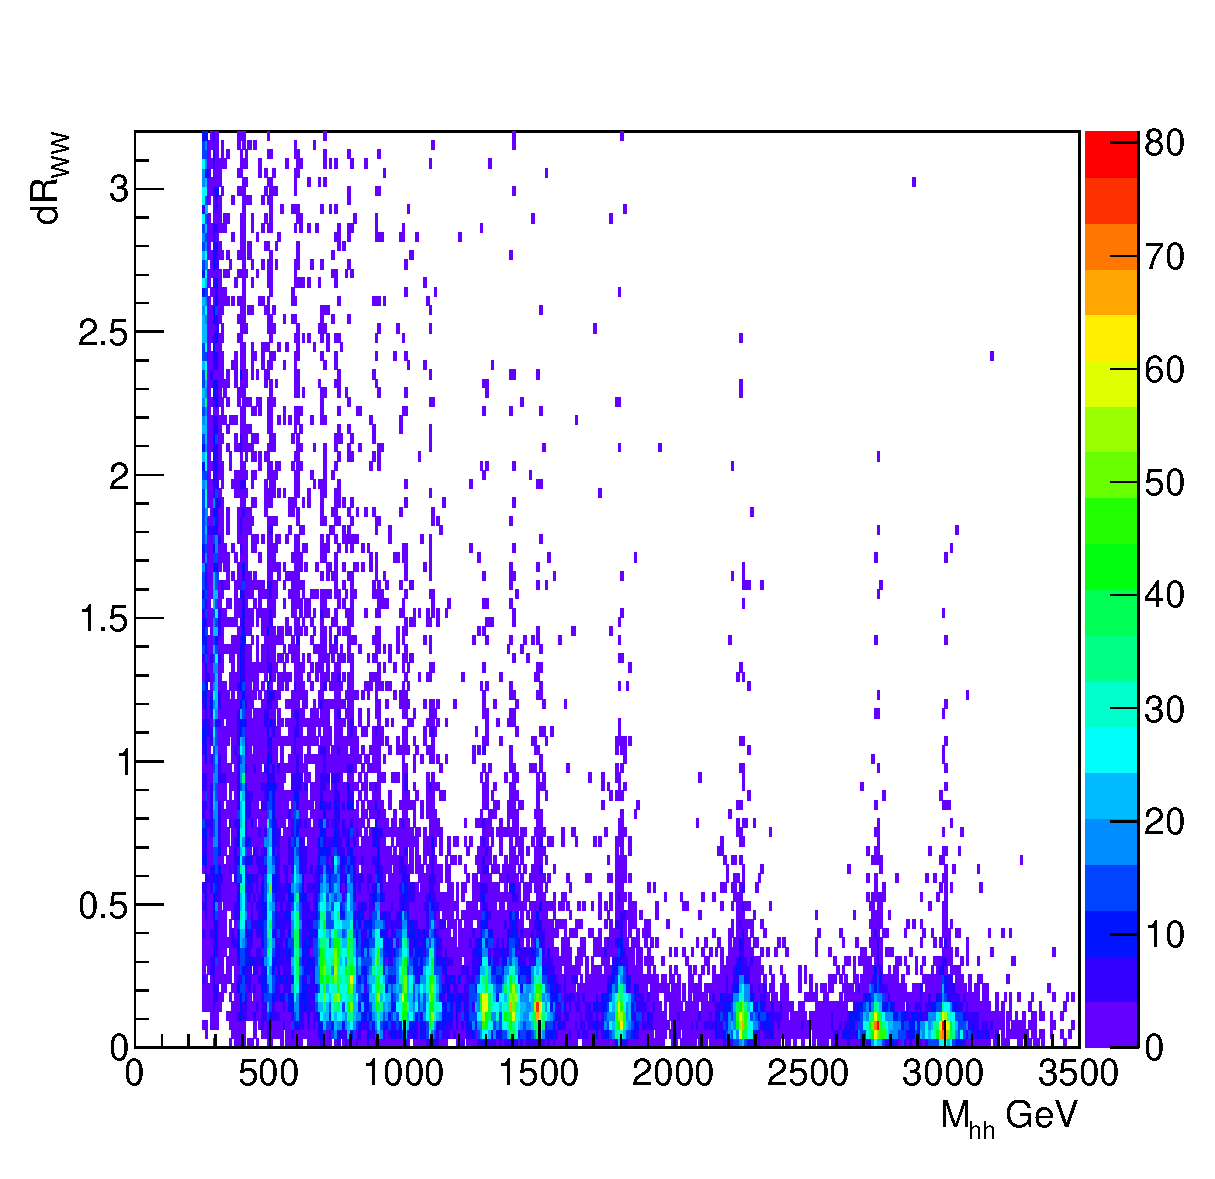
\includegraphics[scale=0.33]{DRMhhPlots_fine/drWW}
\\
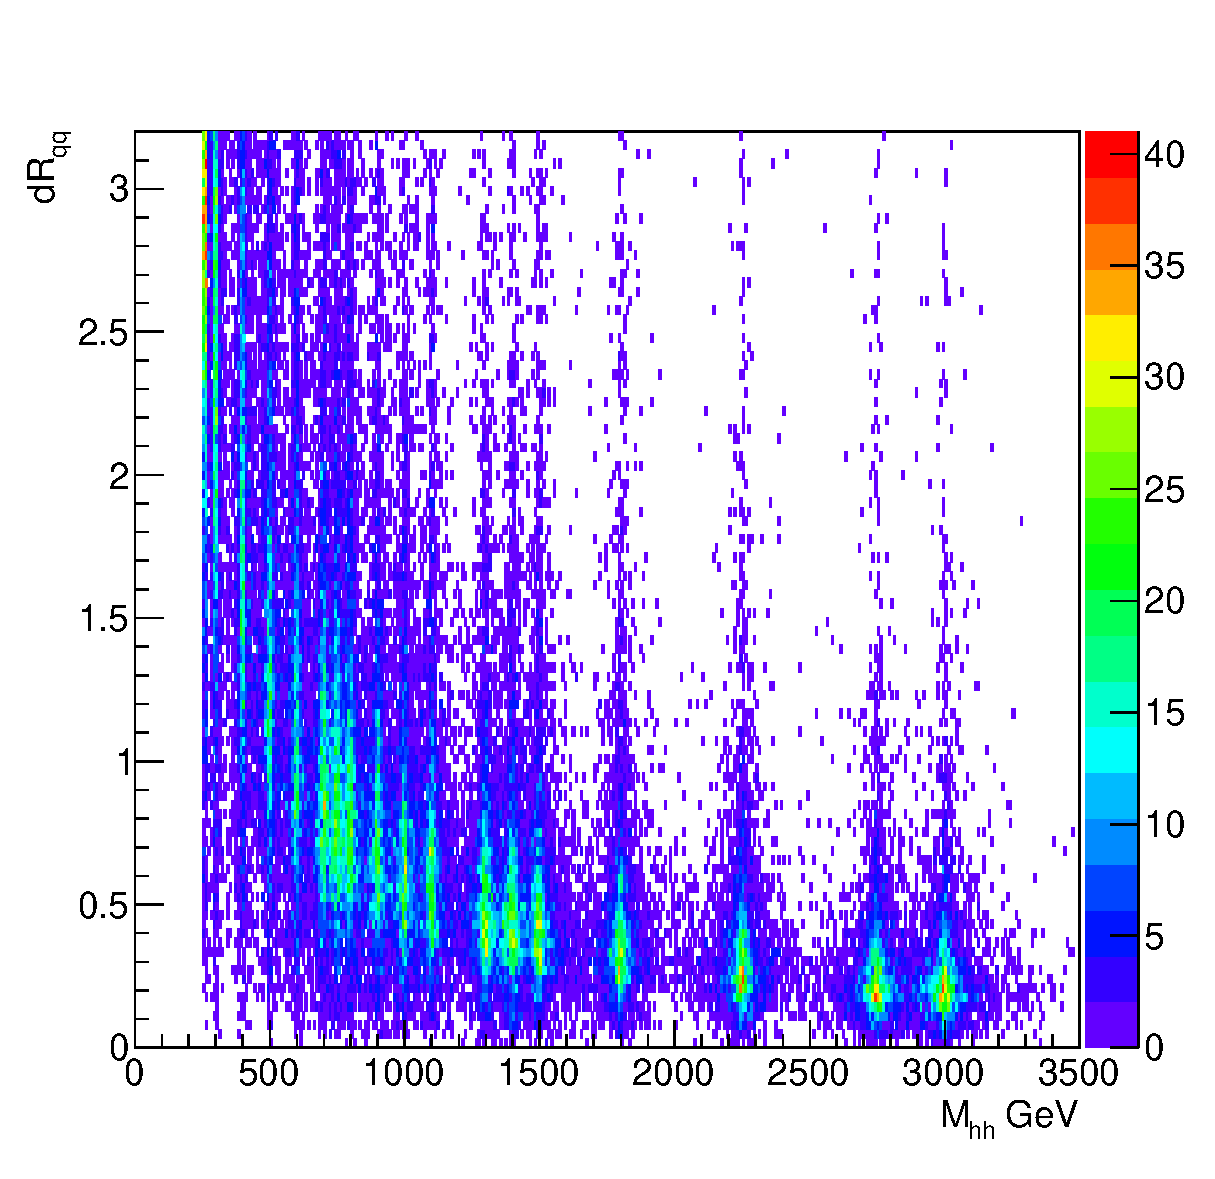
\includegraphics[scale=0.33]{DRMhhPlots_fine/drqq}
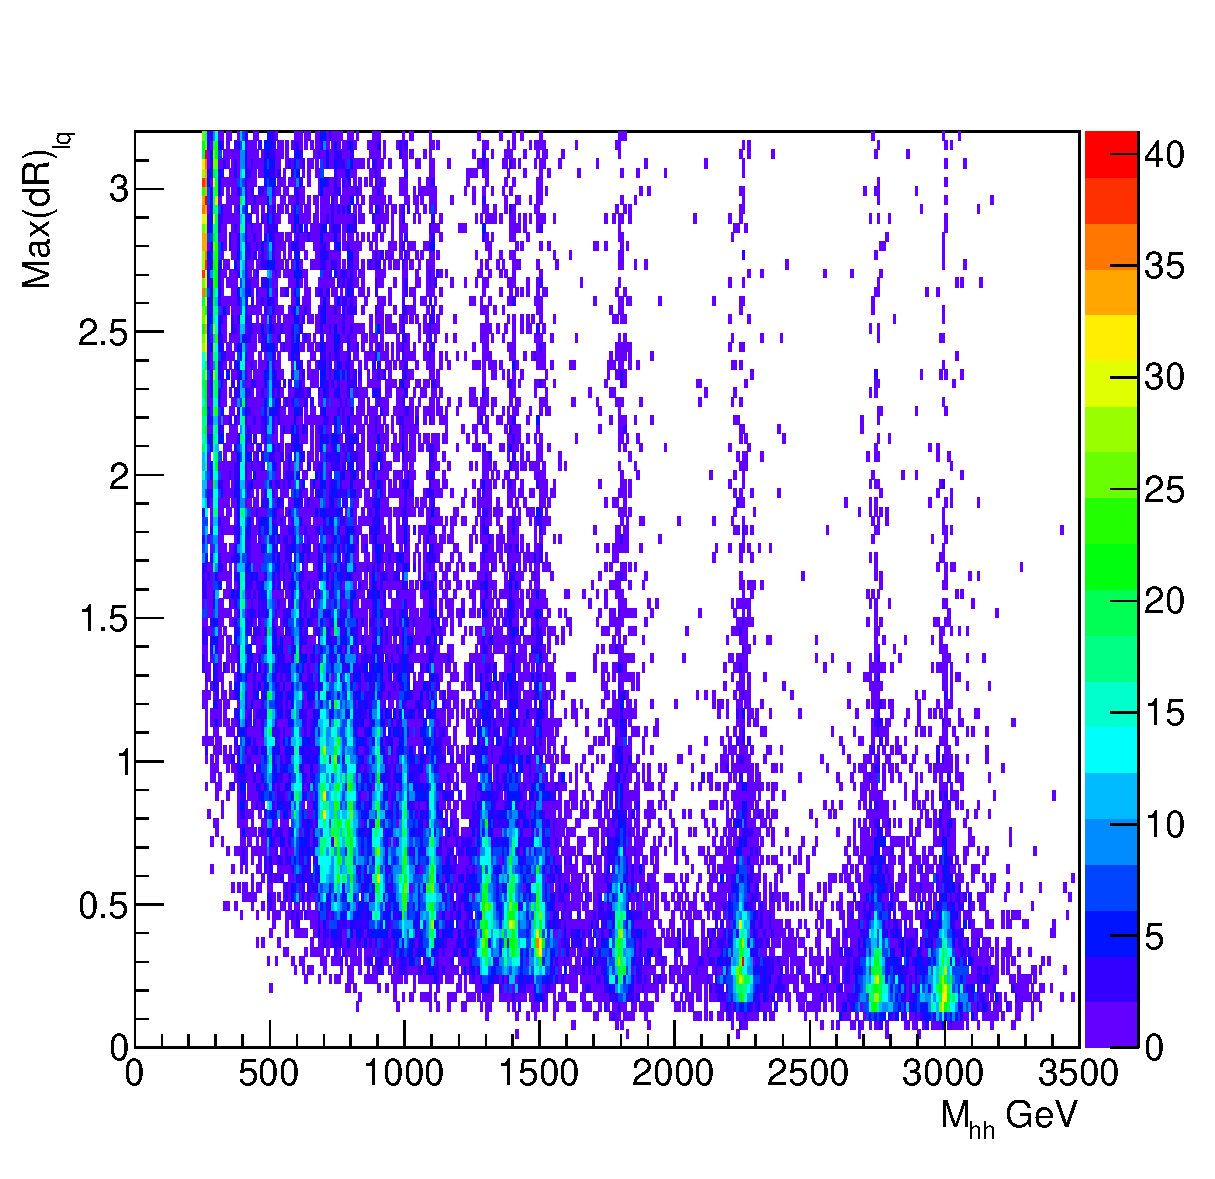
\includegraphics[scale=0.33]{DRMhhPlots_fine/drmaxlq}

\caption{Distance between the two b partons (top left); the two W bosons (top right); the two light quarks (bottom left); and the lepton and the most distant light quark (bottom right) for resonant $HH$ production as a function of resonant mass.}
\label{fig:dr}
\end{center}
\end{figure}
\indent On the ${H\rightarrow b\overline{b}}$ side, this is accounted for through the boosted analysis selection. Moving toward the full Run 2 analysis, it is worth while to look at the potential gain from including a boosted ${H\rightarrow WW^{*}}$ selection. This ``fully-boosted" analysis can be used in conjunction with the current boosted and resolved analysis to increase sensitivity and reach.\newline
%\section{Fully Boosted Analysis}
\indent The ``fully-boosted" analysis piggybacks off of the analysis presented in Chapter ~\ref{chap:anal}. This means the data and Monte Carlo Samples , object reconstruction, and trigger requirements are the same as the previously presented analysis. \newline
\section{Event Reconstruction}
Identically to the boosted analysis, section \ref{sec:Boosted}, events are reconstructed by requiring at least one reconstructed lepton. To reconstruct the ${H\rightarrow b\overline{b}}$ candidate, there should be at least one large-R jet with ${\Delta{R} > 1.0}$ from the selected lepton. The highest of these large-R jets is selected as the ${H\rightarrow b\overline{b}}$ candidate. This large-R jet is then required to have at least to track jets associated to it. Events with a ${H\rightarrow b\overline{b}}$ in the range ${30 \mathrm{GeV} < m_{\mathrm{bb}} < 300 \mathrm{GeV}}$ are retained for further analysis.\newline
\indent To reconstruct the ${H\rightarrow WW^{*}}$ candidate, there should be at least one large-R jet with ${\Delta{R} < 1.0}$ from the selected lepton. This large-R jet is selected as the ${H\rightarrow WW^{*}}$ jet candidate. Once the ${H\rightarrow b\overline{b}}$ jet has been selected, they are split into either electron or muon channel for the full reconstruction.\newline
\indent Calorimeter jets are clusters of energy that are grouped together into an object based on distances. If an electron, which deposits the majority of its energy into the calorimeter, were to fall within the radius of a calorimeter jet, its energy should be measured as part of the jet energy. Using this, it is possible to use a single large-R to measure the energy of the ${W\rightarrow qq}$ system and the electron.  With the large-R jet and the \met, it is possible to fully reconstruct the ${H\rightarrow WW^{*}}$ system. The neutrino is reconstructed using a similar method as in Section ~\ref{ssec:event_reco_res}. Imposing the relation:
\begin{equation}
\label{eq:mh}
m_h^2 = (p^{\nu} + p^{\mathrm{large-R jet}})^2
\end{equation}
the neutrino $p_z$ can be reconstructed using the relations:
\[
p_E^{\nu} = E^{\nu} = \sqrt{P_T^2 + p_z^2} \quad p_x^{\nu} = P_Tcos(\phi) \quad p_y^{\nu} = P_T sin(\phi)
\]
where $\phi$ is the azimuthal angle of the $\met$, $E^{\nu}$ the neutrino energy, $p_x$ and $p_y$ the two transverse spatial components of the neutrino momentum.\newline
\indent Muons do not deposit a significant amount of energy in the calorimeters, this means we cannot use the same reconstruction as for the electrons. Instead, the muons are treated in a more traditional fashion. In the muon channel, the large-R jet contains the energy of the ${W\rightarrow qq}$ system. The muon is reconstructed using the MS and ID information and the neutrino is reconstructed identically to \ref{ssec:event_reco_res}, with the hadronic $W$ as a single object.\newline
\indent Figure ~\ref{fig:topo} shows a diagram of the event topology after the event reconstruction.

\begin{figure}[h]
\begin{center}
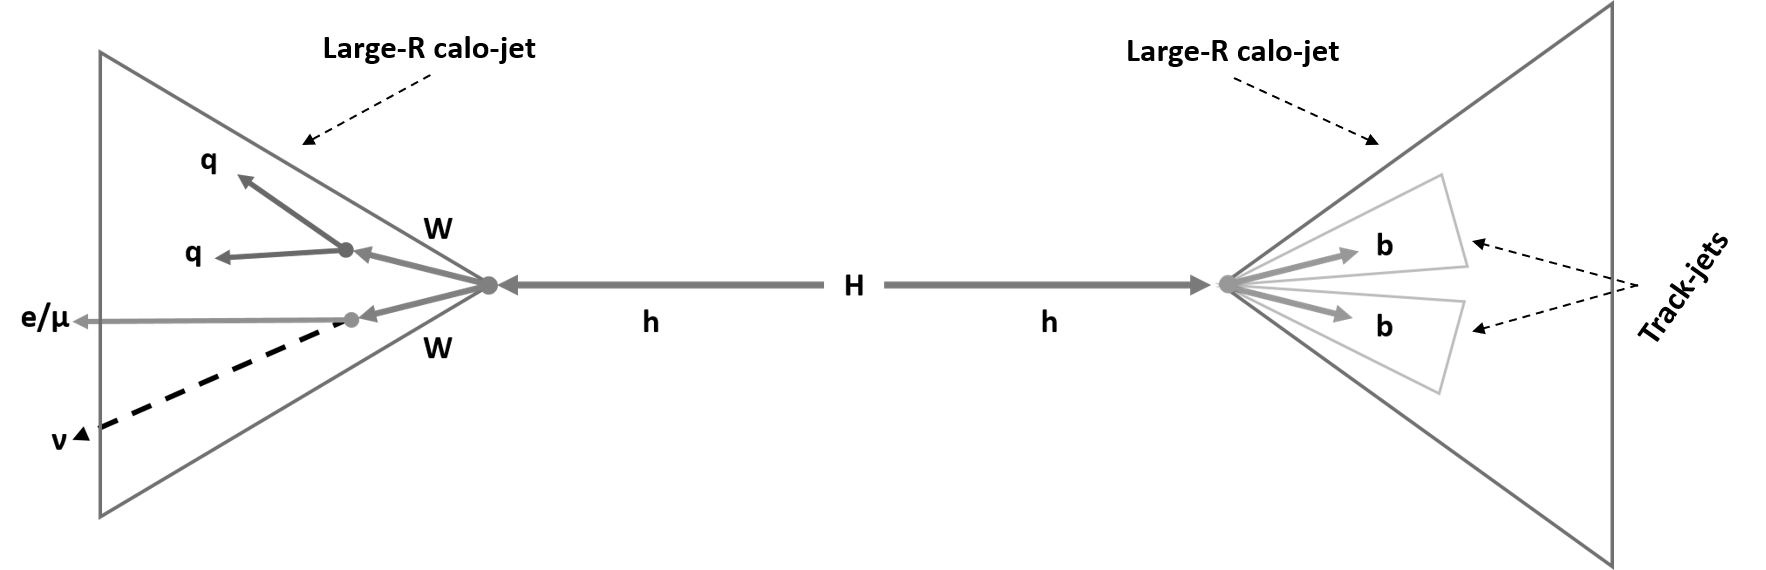
\includegraphics[scale=0.4]{figures/full_boosted}
\caption{Diagram of the fully-boosted event topology}
\label{fig:topo}
\end{center}
\end{figure}
\section{Event selection}
After the event is reconstructed, a b-tag requirement is applied to the 2 track-jets in the ${H\rightarrow b\overline{b}}$ large-R jet. The \met is required to be more than 50 GeV to reject events from QCD background. Finally a  \pt requirement is placed on the ${H\rightarrow WW^{*}}$ candidate. It is important to cut on the same physics objects. To accomplish this, an ``adjusted \pt " (${\pt^{'}}$) cut of 250 GeV is applied. Table ~\ref{tab:adjpt} defines the ${\pt^{'}}$ for both channels. 


\begin{table}
\begin{center}
\begin{tabular}{l|c}
Muon Channel & ${\pt^{'} = \pt^{\mathrm{Large-R jet}}}$\\
\hline
\\
Electron channel & ${\pt^{'} = \sqrt{(p_{x}^{\mathrm{Large-R jet}} - p_{x}^{\mathrm{electron}})^{2}+(p_{y}^{\mathrm{Large-R jet}} - p_{y}^{\mathrm{electron}})^{2}}}$
\end{tabular}
\caption{}
\label{tab:adjpt}
\end{center}
\end{table}

\subsection{Comparison of reconstruction objects}
With this new event reconstruction method and a basic set of cuts, we can compare a few basic kinematic variables to check the performance. Figure XXX shows a comparison of the old boosted analysis reconstruction and the new fully-boosted analysis.

\subsection{Signal Region Definition}
As with the boosted analysis in Section ~\ref{sec:Boosted}, the ${h\rightarrow b\overline{b}}$ candidate must have a jet mass in the window ${90 \mathrm{ GeV } < m_{bb} < 140 \mathrm{GeV}}$ to be considered in the signal region (SR)
\subsection{mBB Control Region}
To check the modeling of the background, a control region is created with an inverted ${m_{bb}}$ cut. 
\subsection{Multijet Background}
The QCD multijet background is estimated using the same data-driven background as the boosted analysis. The ABCD method with the regions defined as:
\begin{itemize}
\item Region A: \met > 50 GeV, $|d_{0}^{\textrm{sig}}|$ $<$ 2.0
\item Region B: \met < 50 GeV, $|d_{0}^{\textrm{sig}}|$ $<$ 2.0
\item Region C: \met > 50 GeV, $|d_{0}^{\textrm{sig}}|$ $>$ 2.0
\item Region D: \met < 50 GeV, $|d_{0}^{\textrm{sig}}|$ $>$ 2.0
\end{itemize}

\subsubsection{Yield Prediction}
Table \ref{tab:boosted_region_bd_promptbkgd_data_new} lists the MC predicted prompt lepton backgrounds, observed data and calculated multijet yields in Region B and D before the ${H\rightarrow b\overline{b}}$ mass cut is applied and Table \ref{tab:boosted_region_c_promptbkgd_data_new} shows the yields in Region C mBB control region and signal region.\newline

\begin{table}
\begin{center}
\begin{tabular}{l|c|c||c|c}
             &\multicolumn{2}{c||}{Region B}                &\multicolumn{2}{c}{Region D} \\
\hline
Samples       & Electron               & Muon                & Electron          & Muon \\      
\hline
$t\bar{t}$    &  138.7 $\pm$ 7.3      & 146.1 $\pm$ 8.3      & 14.4 $\pm$ 2.7    & 6.3  $\pm$ 1.5  \\
W+Jets        &  27.3 $\pm$ 1.7       & 27.9 $\pm$ 1.9       & 1.1 $\pm$ 0.3    & 2.0  $\pm$ 0.4  \\        
Single-top    &  7.1  $\pm$ 1.4       & 5.2  $\pm$ 1.4     &  0.2 $\pm$ 0.2    &  0.4  $\pm$ 0.3  \\
Z+Jets        &  18.3  $\pm$ 0.8       & 9.3  $\pm$ 0.5     &  1.9 $\pm$ 0.3    &  0.9  $\pm$ 0.2  \\
Dibosons      &  3.1  $\pm$ 0.5       & 1.3  $\pm$ 0.3     &  0.2 $\pm$ 0.1    &  0.2  $\pm$ 0.1  \\
\hline
Total Prompt  &  194.4 $\pm$ 7.7      & 189.9 $\pm$ 8.7    & 17.8 $\pm$ 2.7    & 9.8  $\pm$ 1.6  \\
\hline
Data          &  274.0  $\pm$ 16.6      & 218.0   $\pm$ 14.8    & 34.0  $\pm$ 5.8   & 30.0   $\pm$ 5.5  \\
\hline
QCD           & 79.6 $\pm$ 18.3       & 28.1 $\pm$ 17.1    & 16.2 $\pm$ 6.4  & 20.2 $\pm$ 5.7 \\
\end{tabular}
\end{center}
\caption{MC predicted prompt lepton backgrounds, observed data and calculated multijet yields
in Region B and D. The multijet yield is calculated by subtracting the estimated total prompt lepton
backgrounds from the observed data. The statistical uncertainty on the yields is shown.}
\label{tab:boosted_region_bd_promptbkgd_data_new}
\end{table}


\begin{table}
\begin{center}
\begin{tabular}{l|c|c||c|c}
             &\multicolumn{2}{c||}{mBBcr}               &\multicolumn{2}{c}{SR}\\
\hline
Samples       & Electron            & Muon               & Electron         & Muon     \\      
\hline
$t\bar{t}$          &   21.7	$\pm$ 4.1   &   12.8 $\pm$ 2.1	&  	6.4 $\pm$ 1.4		& 	5.4 $\pm$ 1.2\\
W+Jets          &   3.4 	$\pm$ 0.6   &    2.3 $\pm$ 0.3	&	1.4 $\pm$ 0.3		&  	1.2 $\pm$ 0.3\\
Single-top      &   0.7 	$\pm$ 0.5   &    0.3 $\pm$ 0.2	&	0.4 $\pm$ 0.3       	&  	0.2 $\pm$ 0.2\\
Z+Jets          &   1.0 	$\pm$ 0.2   &    0.4 $\pm$ 0.1	& 	0.4 $\pm$ 0.1        & 	0.2 $\pm$ 0.1\\
Dibosons   &   0.2 	$\pm$ 0.1   &    0.0 $\pm$ 0.0	&	0.1 $\pm$ 0.1       	& 	0.0 $\pm$ 0.0\\
\hline
Total Prompt         &   26.9 	$\pm$ 4.1   &   15.9 $\pm$ 2.2	&	8.7 $\pm$ 1.5       	& 	7.0 $\pm$ 1.3\\
\hline
Data           &   53.0 $\pm$ 7.3   &   33.0 $\pm$ 5.7	&	12.0 $\pm$ 3.5      	& 	20.0 $\pm$ 4.5\\
\hline
QCD            &   26.1 $\pm$ 8.4   &   17.1 $\pm$ 6.1	&	3.3 $\pm$ 3.8       	& 	13.0 $\pm$ 4.7\\
\end{tabular}
\end{center}
\caption{MC predicted prompt lepton backgrounds, observed data and calculated multijet yields
in Region C mBBcr and SR. The multijet yield is calculated by subtracting the estimated total prompt lepton
backgrounds from the observed data. The statistical uncertainty on the yields is shown.}
\label{tab:boosted_region_c_promptbkgd_data_new}
\end{table}


\indent Table XXX shows the ratio in the electron channel and muon channel.
The predicted yields of the QCD multijet background in the mBB control region and signal region are presented in table XXX. The QCD multijet background is estimated to be XXX\% of the total background in the signal region (Table XXX).

\begin{table}
\begin{center}
\begin{tabular}{c|c|c}
Multijet yield in region              & Electron                & Muon   \\      
\hline
$N_B^\text{QCD}$                      & 79.6 $\pm$ 18.3      & 28.1 $\pm$ 17.1 \\
$N_D^\text{QCD}$                      & 16.2 $\pm$ 6.4      & 20.2 $\pm$ 5.7  \\
\hline
$N_{B}^\text{QCD}$/$N_{D}^\text{QCD}$     & 4.9 $\pm$ 2.62 (46.0\%) & 1.4 $\pm$ 0.94 (67.2\%)   \\
\end{tabular}
\end{center}
\caption{Multijet yields in region B and region D and also the ratio of the yields for each lepton channel. The error
on the $\frac{N_B^\text{QCD}}{N_D^\text{QCD}}$ ratio is propagated from the statistical uncertainties on the multijet yields in each region.}
\label{tab:boosted_bkgd_abcd_ratio_new}
\end{table}

\begin{table}[!htbp]
\begin{center}
\begin{tabular}{c|c|c}
Multijet yield in region & Electron  & Muon  \\  
\hline
\multicolumn{3}{c}{SR} \\
\hline
$N_C^\text{QCD}$         & 3.3  $\pm$ 3.8 & 13.0 $\pm$ 4.7 \\
$N_A^\text{QCD}$         & 16.4 $\pm$ 20.5 (126.8\%) & 18.1 $\pm$ 13.9 (76.8\%) \\
\hline
\multicolumn{3}{c}{mBBcr} \\
\hline
$N_C^\text{QCD}$       & 26.1  $\pm$ 8.4 & 17.1  $\pm$ 6.1  \\
$N_A^\text{QCD}$       & 128.3 $\pm$ 79.4 (61.9\%) & 23.9 $\pm$ 18.1 (75.7\%)  \\
\hline
\end{tabular}
\end{center}
\caption{Multijet yield in region C and predicted yield in region A in the SR. The error on $N_A^\text{QCD}$
are propagated from the error on the $N_B^\text{QCD}$/$N_D^\text{QCD}$ ratio and statistical uncertainty on $N_C^\text{QCD}$ yield.
The numbers in brackets are the relative uncertainty in percentage.}
\label{tab:boosted_bkgd_abcd_yield_new}
\end{table}


\subsubsection{Shape prediction}
See Section \ref{sec:boosted_bkgd_qcdmultijet_shape}.

\subsubsection{Multijet yield uncertainties}
\label{sec:boosted_bkgd_qcdmultijet_yield_unc}
 
%%%%%%%%%%%%%%%%%%%%%%%%%%%%%%%
% Statistical
%%%%%%%%%%%%%%%%%%%%%%%%%%%%%%%
\paragraph{Statistical} 
The uncertainty on the predicted yield of the multijet background is determined by propagating the statistical uncertainty
of the $\frac{N_B^\text{QCD}}{N_D^\text{QCD}}$ ratio, as shown in Table~\ref{tab:boosted_bkgd_abcd_ratio_new}, and the statisical
uncertainty on the multijet yield in region C ($N_C^\text{QCD}$), as in Table~\ref{tab:boosted_bkgd_abcd_yield_new}.
 
\paragraph{1-tag/2-tag jet mass acceptance} 
Another source of uncertainty on the multijet yield is the  
the difference of acceptance of the large-$R$ jet mass cut between 1-tag and 2-tag.
This uncertainty is included since the template for or the multijet shape prediction uses the multijet shape
from the 1-tag region C. Table~\ref{tab:boosted_syst_qcd_norm_mBBAcc} shows the acceptance
of the large-$R$ jet mass signal and mBB control region selection in the multijet 1-tag region C and 2-tag region C yields.
The relative difference between the acceptance in 1-tag region C and in 2-tag region C is considered as an uncertainty on the normalization
of the QCD multijet prediction.
 
\begin{table}[!htbp]
\begin{center}
\begin{tabular}{c|c|c}
\hline
Region    & Electron          & Muon      \\
\hline
\multicolumn{3}{c}{SR} \\
\hline
1-tag $\frac{N_\text{SR}}{N_\text{Inc}}$ &  32\% & 23 \% \\
2-tag $\frac{N_\text{SR}}{N_\text{Inc}}$ &  11\% & 43 \% \\
\hline \hline
Rel. difference between 1-tag and 2-tag & 26.4 \% & 46 \% \\
\hline
\multicolumn{3}{c}{mBBcr} \\
\hline
1-tag $\frac{N_\text{mBBcr}}{N_\text{Inc}}$ &  68\% & 77 \% \\
2-tag $\frac{N_\text{mBBcr}}{N_\text{Inc}}$ &  89\% & 56 \% \\
\hline \hline
Rel. difference between 1-tag and 2-tag &  24 \% &   37 \% \\
\end{tabular}
\end{center}
\caption{The acceptance of the large-$R$ jet mass signal region selection on the multijet
1-tag and 2-tag region C. $N_\text{SR}$($N_\text{Inc}$) is the multijet yield
with (without) the signal region large-$R$ jet mass selection.}
\label{tab:boosted_syst_qcd_norm_mBBAcc}
\end{table}
 

%%Yields in ABCD regions, 


\subsubsection{Hadronic ${WW^{*}}$ \pt}